\section{Preparation}

\noindent
This chapter covers the following ideas. When you create your lesson plan, it should contain examples which illustrate these key ideas. Before you take the quiz on this unit, meet with another student out of class and teach each other from the examples on your lesson plan. 


\begin{enumerate}

\item Create examples to illustrate mathematical definitions. Know these definitions.
\item Create examples to illustrate theorems. You do not have to memorize all the theorems, rather when one is given make sure you can construct examples of it. 
\item When a matrix has an inverse, this is equivalent to many other facts about the matrix and corresponding systems of equations.  Illustrate this equivalence with examples, and be able to explain why the the ideas are equivalent.
\item Be able to explain why something is or is not a vector space. Give examples of vector spaces and subspaces that you have encountered previously in this class and other classes.
\item Explain how to find a basis for a vector space and the dimension of a vector space. Give the coordinates of vectors relative to a chosen basis.

\end{enumerate}


Here are the preparation problems for this unit.  Problems that come from Schaum's Outlines ``Beginning Linear Algebra'' are preceded by a chapter number. From here on out, many of the problems we will be working on come from Schaum's Outlines.  Realize that sometimes the method of solving the problem in Schaum's Outlines will differ from how we solve the problem in class. The difference is that in Schaum's Outlines they almost always place vectors in rows prior to row reduction, whereas we will be placing vectors in columns. There are pros and cons to both methods. 


\begin{center}
\begin{tabular}{ll}
\multicolumn{2}{c}{Preparation Problems
  (\href{http://ilearn.byui.edu/bbcswebdav/institution/Physical\_Sci\_Eng/Mathematics/Personal\%20Folders/WoodruffB/341/3-Patterns-Preparation-Solutions.pdf}{click
    for handwritten solutions})}
\\
\hline\hline
Day 1&
1f,
2a,
2f,
2i
\\ \hline
Day 2&
2j,
4b,
Chp 4:6
Chp 4:13
\\ \hline
Day 3&
Chp 4:22
Chp 5:18
Chp 6:6
Chp 6:9
\\ \hline
Day 4&
Lesson Plan,
Quiz, Start Project 
\\ \hline
\end{tabular}
\end{center}


\subsection{Webcasts}

\href{http://www.youtube.com/user/bmwoodruff\#g/c/54D7F4A63AE6AE18}{Click
  here for webcasts on YouTube}\footnote{\url{http://www.youtube.com/user/bmwoodruff\#g/c/54D7F4A63AE6AE18}}.  \href{http://ilearn.byui.edu/bbcswebdav/institution/Physical\_Sci\_Eng/Mathematics/Personal\%20Folders/WoodruffB/341/3-Patterns-videos.pdf}{Click
  here for a pdf copy of the papers in the webcasts}.

\subsection{Suggested Problems}

The first three sets of problems are in this book.  The remaining problems come from Schaum's Outlines ``Beginning Linear Algebra'' by Seymour Lipschutz.  
\begin{center}
\begin{tabular}{|l|l|l|l|l|}
\hline
Concept&Suggestions&Relevant Problems\\ \hline
Illustrating Definitions
	&\ref{definition problems}cdf
  &\ref{definition problems}
  \\ \hline
Illustrating Theorems
	& \ref{theorem problems}acdfijl (all are good)  
	&\ref{theorem problems}
	\\ \hline
The huge equivalence
	&\ref{equivalence problems}abe 
	&\ref{equivalence problems}
	\\ \hline
Vector Spaces
	& In Schaum's
	&\ref{vector space problems}
	\\ \hline
Subspaces
	& In Schaum's
	&\ref{subspace problems}
	\\ \hline
Spans
	&In Schaum's
	&\ref{span problems}
	\\ \hline
Basis and Dimension
	&In Schaum's
	&\ref{basis problems}
	\\ \hline
Coordinates
	&In Schaum's
	&\ref{coordinates problems}
	\\ \hline
Linear Independence
	&In Schaum's
	&\ref{independence problems}
	\\ \hline
\end{tabular}
\end{center}

%%% Local Variables: 
%%% mode: latex
%%% TeX-master: "../linear-algebra"
%%% End: 


\section{Problems}

Much of the point to this section is to learn to read mathematics and create examples to illustrate definitions and theorems.  
For this reason, each problem below requires reading and working with different definitions and theorems. The common theme to the problems is that you are to create examples.  The latter half of the problems are in you Schaum's Outlines  ``Beginning Linear Algebra'' book.


\begin{enumerate}


\item \textbf{Illustrating Definitions:} \label{definition problems}
For this problem you are creating examples to illustrate a definition. If actual vectors or matrices are given, use them to illustrate the definition. Then create your own example using your own vectors and/or matrices.

\begin{enumerate}
	\item Give an example of a pair of nonzero vectors that are orthogonal. Also give an example of a pair of vectors that are not orthogonal. Draw your vectors to show that the angles meet at a 90 degree angle.
	\item Give an example of a matrix that is in row echelon form but not reduced row echelon form. Then give the reduced row echelon form of the matrix. 
	\item Show that the set of vectors $\{(1,1,0),(1,0,1),(0,1,1)\}$ is linearly independent by showing that the only solution to $c_1(1,1,0)+c_2(1,0,1)+c_3(0,1,1)=(0,0,0)$ is the trivial solution. Then select your own 3 vectors in 3D and determine if they are independent or dependent.  
	\item Consider the matrix 
	$A=\begin{bmatrix}
	1 & 2 & 0 & 3 \\
	2 & 4 & 0 & 6 \\
	-1 & 3 & 2 & 0
	\end{bmatrix}$ 
	Find a basis for the column space and row space of A. What are the coordinates of each column relative to your basis vectors for the column space?  Now select your own 3 by 4 matrix and repeat this problem.
	\item Show that the inverse of 
	$A=
\begin{bmatrix}
 -2 & 0 & 5 \\
 -1 & 0 & 3 \\
 4 & 1 & -1
\end{bmatrix}
$
is 
$B=
\begin{bmatrix}
 -3 & 5 & 0 \\
 11 & -18 & 1 \\
 -1 & 2 & 0
\end{bmatrix}
$ by computing both $AB$ and $BA$. Now select your own 3 by 3 matrix $A$ and use software to find the inverse $B$ as well as compute $AB$ and $BA$ to verify that $B$ is the inverse.

	\item 
Consider the matrix $A=\begin{bmatrix}2&1&4\\ 1&2&4\\ 0&0&1\end{bmatrix}$. Compute $A\vec x$ for each of the 4 vectors 
$\vec x_1 =(-1,1,0)$, $\vec x_2=(2,0,3)$, $\vec x_3=(1,1,0)$, and $\vec x_4=( -4,0,1)$ to determine which are eigenvectors. 
If a vector is an eigenvector, state the corresponding eigenvalue. 
Now select your own 3 by 3 matrix $A$ and use software to find a basis for the eigenspace (you may have to play with the numbers a little to get simple vectors - or grab an example from earlier in the text where you know the answer). For each vector in the eigenspace, compute $A\vec x$ and verify that $A\vec x = \lambda \vec x$. 



\end{enumerate}




\item \textbf{Illustrating Theorems:}  \label{theorem problems}
Follow the instructions for each problem.  For most of the problems below, you will start with a matrix and then use that matrix to illustrate several theorems from the theorem section of the textbook.  After you have done so with the examples provided, you should select your own matrix and repeat the illustration.

\begin{enumerate}
	\item Which of the following 3 matrices are row equivalent? 
	$$
	A = 
	\begin{bmatrix}
	1 & 1 & 5 \\
	2 & 3 & 13\\
	1 & 2 & 8
	\end{bmatrix}
	B = 
	\begin{bmatrix}
	1 & -1 & -2 \\
	3 & -2 & -3 \\
	-1& 0  & -1
	\end{bmatrix}
	C = 
	\begin{bmatrix}
	1 & -1 & -1 \\
	4 & -3 & -1 \\
	3 & -1 & 3	
	\end{bmatrix}.
	$$
	By row reducing each matrix, use theorem \ref{thm row equivalent} to make your decision. 
	
	Now try problem 4.22 on page 172 in Schaum's outlines.  
	 
	\item Consider the non homogeneous system of equations $x+2y+4w=4, 2x+3y-z=-1, 3x+5y-z+4w=3$, written in matrix form as 
	$
	\begin{bmatrix}
	1 & 2 & 0 & 4 \\
	2 & 3 & -1 & 0\\
	3 & 5 & -1 & 4	
	\end{bmatrix}
	\begin{bmatrix}
	x\\y\\z\\w	
	\end{bmatrix}
	=\begin{bmatrix}
	 4\\
	 -1\\
	 3	
	\end{bmatrix}
	$.  
	Use theorem \ref{thm solution iff augmented not pivot} to decide if there is a solution to this equation. 
	How many free variables are there based on theorem \ref{thm n-k free variables}? 
	Find two different solutions $\vec x_1$ and $\vec x_2$ to this system (let $z=1,w=0$ and $z=0,w=1$).  
	Compute $A(\vec x_1 - \vec x_2)$ and use your result to verify \ref{thm non homogeneous}. 
	
	Now create your own 3 by 5 augmented matrix and repeat this problem. 
	
	\item Consider the homogeneous system of equations $x+2y+4w=0, 2x+3y-z=0, 3x+5y-z+4w=0$, written in matrix form as 
	$
	\begin{bmatrix}
	1 & 2 & 0 & 4 \\
	2 & 3 & -1 & 0\\
	3 & 5 & -1 & 4	
	\end{bmatrix}
	\begin{bmatrix}
	x\\y\\z\\w	
	\end{bmatrix}
	=\begin{bmatrix}
	 0\\
	 0\\
	 0	
	\end{bmatrix}
	$.  
	How many free variables are there based on theorem \ref{thm n-k free variables}?
	Find two different solutions $\vec x_1$ and $\vec x_2$ to this system (let $z=1,w=0$ and $z=0,w=1$).  
	Illustrate theorem \ref{thm homogeneous} by computing $A(\vec x_1 + \vec x_2)$. 
	
	Now create your own homogeneous system and repeat this problem. 	
	
	\item Consider the two matrices 
	$A=
	\begin{bmatrix}
	 1 & 2 & 3\\
	 4 & 5 & 6
	\end{bmatrix}
	, 
	B=
	\begin{bmatrix}
	 2\\-1\\3
	\end{bmatrix}$. Verify theorem \ref{thm transpose of product}  by computing $AB$, $(AB)^T$, $A^TB^T$ and $B^TA^T$ (notice that $A^TB^T$ doesn't even make sense). 
	
	Now repeat this problem with two matrices such that the product $AB$ makes sense.
	
	
	\item Use the same two matrices from the previous problem to illustrate theorem \ref{matrix multiplication two ways}. Table \ref{matrixmult} on page \pageref{matrixmult} contains another example.  
	
	Now select two matrices of your own and repeat this problem.
	
	
	
	\item Consider the matrix $A=\begin{bmatrix}
	1 & 2 & 0 & 4 \\
	2 & 3 & -1 & 0\\
	3 & 5 & -1 & 4	
	\end{bmatrix}$. Find the rref of $A$. Use theorem \ref{thm rank equal pivot columns} to determine the rank of $A$. Use theorem \ref{every column pivot iff independent} to determine if the columns are linearly independent. Use theorem \ref{thm colsp basis} to give a basis for the column space as well as the coordinates of each column of $A$ relative to this basis.  Use theorem \ref{thm rowsp basis} to give a basis for the row space of $A$ as well as the coordinates of each row of $A$ relative to this basis. Are the dimensions of the column and row space the same (as theorem \ref{rankrowcolumn} suggests)? 
	
	Now repeat this problem with a matrix of your own. 
	
  \item Let 
  $A=\begin{bmatrix}
	1 & 2 \\
	3 & 5
	\end{bmatrix}$.  
	Find the inverse of $A$ by row reducing $[A|I]$.  
	Then find the inverse of $A\inv$ by row reducing $[A\inv|I]$ to illustrate theorem \ref{thm inverse of inverse}.  
	Now compute $(A^T)\inv$ and $(A\inv)^T$ to illustrate theorem \ref{thm inverse of transpose}.
	
  Repeat this problem with a 2 by 2 or 3 by 3 matrix of your own.
  
  
  \item Consider the matrices 
    $A=\begin{bmatrix}
	1 & 2 \\
	3 & 5
	\end{bmatrix}$ and 
	  $B=\begin{bmatrix}
	3 & 2 \\
	4 & 3
	\end{bmatrix}$.
	Illustrate theorem \ref{invprod} by computing $A\inv$, $B\inv$, $(AB)\inv$, and $B\inv A\inv$. 
  
  Repeat this on a pair of 2 by 2 or 3 by 3 matrices of your own.

  \item  Consider the triangular 4 by 4 matrix 
  $A=\begin{bmatrix}
	1 & 8 & -12& 0 \\
	0 & 2 & 5& 16 \\
	0 & 0 & -3& -4 \\
	0 & 0 & 0& 4
	\end{bmatrix}$.  
	Find the determinant of $A$ (make sure you use a cofactor expansion along columns that contain lots of zeros). Similarly find the characteristic polynomial of $A$ (the determinant of $A-\lambda I$). The polynomial should already be factored, so find the eigenvalues of $A$. Compare your results to theorems \ref{thm det triangular} and \ref{thm eigen triangular}.
	
	Now select a 4 by 4 or 5 by 5 triangular matrix and repeat this problem.
  
  \item Consider the 3 by 3 matrix 
  $A = 
\begin{bmatrix}
1&2&0\\
-1&3&4\\
2&-3&1
\end{bmatrix}
$. 
  Find the determinant of $A$ by using a cofactor expansion along row 1. 
  Now find the determinant of $A^T$ by using a cofactor expansion along column 1. Why does your work verify  theorem \ref{thm det transpose}? 
  Show that the characteristic polynomial of $A$ and $A^T$ is the same by computing the determinants of $A-\lambda I$ and $A^T-\lambda I$ using the first row and first column.
  Why does this imply theorem \ref{thm eigen transpose}. Notice that without even computing the eigenvalues, we can conclude that they are the same for $A$ and $A^T$ because the characteristic polynomials are the same.

Repeat this problem on a different 3 by 3 matrix.
  
  \item Consider the matrix 
  $A = 
\begin{bmatrix}
1&2&3\\
-1&3&-3\\
2&4&6
\end{bmatrix}
$. Compute the determinant of $A$.  Now use theorem \ref{thm det multiple columns} to explain why the determinant is zero. Use theorem \ref{thm det zero} to explain why $A$ has no inverse.
  
  Create a 4 by 4 matrix in which one row is a multiple of another row. Then repeat this problem. 
  
  \item Consider the matrix 
  $A = 
\begin{bmatrix}
1&2&0\\
1&3&0\\
4&-1&2
\end{bmatrix}
$. 
Compute each of the cofactors of $A$. Find the adjoint of $A$ (place the $C_{ij}$ cofactor in the $i$th column, $j$th row). Let $B=\frac{1}{|A|}\text{adj}(A)$. Show by computing $AB$ that $B$ is the inverse of $A$ (theorem \ref{thm adjoint}).

Pick another 3 by 3 matrix that has an inverse, and repeat this problem.
	

	\item Consider the matrix   $A = 
\begin{bmatrix}
1&2&-4&3\\
1&3&7&-9\\
-4&-1&2&5\\
0&3&-4&3
\end{bmatrix}
$. 
What is the sum of each row of $A$? Show that $\vec x = (1,1,1,1)$ is an eigenvector of $A$ by computing $A\vec x$. What is the corresponding eigenvalue (it should be the sum of each row)? You have essentially showed why theorem \ref{thm eigenvalues and sums} is true. Use theorem \ref{thm eigen transpose} to decide if $\lambda=2$ is an eigenvalue of $A^T$. [This problem is why $\lambda =1 $ is an eigenvalue of the transition matrices in a Markov process.]
	
	Create a 4 by 4 matrix where each row sums to the same number.  Repeat the computations above.
	
	\item Consider the symmetric matrix 
  $A = 
\begin{bmatrix}
2&1&0\\
1&2&0\\
0&0&4
\end{bmatrix}
$. 
Find the 3 distinct eigenvalues of $A$, and a basis vector for each corresponding eigenspace. Find the dot product of each pair of vectors and compare your result to theorem \ref{thm spectral}.  Show that the three eigenvectors are linearly independent  as theorem \ref{thm independent eigenvectors} suggests (rref a matrix with these eigenvectors as column vectors).

	Repeat this problem with another symmetric matrix. 
\end{enumerate}













\item \textbf{Proving Theorems:} Prove the following theorems. (We will not be focusing on this in our class.)












\item \textbf{A Huge Equivalence:}  
Illustrate Theorem \ref{huge equivalence} \label{equivalence problems} (the huge equivalence) with the following matrices.  First determine if the matrix is singular or nonsingular, and then verify the 11 items from the theorem. Feel free to use a computer to do your computations.
\begin{enumerate}
\begin{multicols}{4}
	\item $\begin{bmatrix} 2&1\\3&4\end{bmatrix}$
	\item $\begin{bmatrix} 2&1\\4&2\end{bmatrix}$
	\item $\begin{bmatrix} 2&1&3\\1&2&4\\0&0&3 \end{bmatrix}$
	\item $\begin{bmatrix} 2&1&3\\1&2&4\\0&-3&-5 \end{bmatrix}$
\end{multicols}
	\item Create your own 3 by 3 or 4 by 4 matrix. Illustrate the theorem with this matrix.
\end{enumerate}




\item \textbf{Vector Spaces:}  \label{vector space problems}
See chapter 4 problems 1-6, 38. Complete at least 6, 38. 


\begin{enumerate}
	\item Show that the set $M_{22}$ of 2 by 2 matrices using  regular matrix addition and regular scalar matrix multiplication is a vector space by showing that it satisfies all 8 axioms.
	\item Let $V$ be the set of real valued functions $y=f(x)$ defined on the entire real number line. Define vector addition as function addition $(f+g)(x) = f(x)+g(x)$, and scalar multiplication as $(cf)(x) = c(f(x))$. Show that $V$ is a vector space with these two operations. 
	
	Could you have changed ``the entire real number line'' to any interval?
	
	\item This example shows that vector addition and multiplication can be defined in very different ways and still result in a vector space. Let $V$ be the set of vectors $(a,b)$ in the plane such that both $a>0$ and $b>0$. If $(a,b)$ and $(c,d)$ are elements of $V$, define vector addition to be $(a,b)+(c,d) = (ac,bd)$.  Define scalar multiplication by a real number $x$ to be $x(a,b) = (a^x, b^x)$.  Show that $V$ is a vector space with zero vector $(1,1)$.

	\item Let $V$ be the set of vectors $(a,b)$ in $\mathbb{R}^2$. If we use regular vector addition but redefine scalar multiplication to be $k(a,b) = (2ka,2kb)$, does this make $V$ a vector space? (Check the 4 axioms related to scalar multiplication.)
	
	\item Let $V$ be the set of vectors $(a,b)$ in $\mathbb{R}^2$. Explain why the following ways of defining vector addition and scalar multiplication do not make $V$ a vector space. Find an axiom that is not satisfied.
\begin{enumerate}
	\item Usual addition $(a,b)+(c,d) = (a+c,b+d)$, but define scalar multiplication as $k(a,b) = (a,kb)$.
	\item Define addition $(a,b)+(c,d) = (a+c,b)$, and use regular scalar multiplication $k(a,b) = (ka,kb)$. 
\end{enumerate}


	\item Let $V$ be the set of vectors $(a,b)$ in $\mathbb{R}^2$. Explain why the following ways of defining vector addition and scalar multiplication do not make $V$ a vector space. Find an axiom that is not satisfied.
\begin{enumerate}
	\item Usual addition $(a,b)+(c,d) = (a+c,b+d)$, but define scalar multiplication as $k(a,b) = (k^2a,kb)$.
	\item Define addition $(a,b)+(c,d) = (a,d)$, and use regular scalar multiplication $k(a,b) = (ka,kb)$. 
\end{enumerate}


\end{enumerate}

\item \textbf{Vector Subspaces:}  \label{subspace problems}
See chapter 4 problems 13-15, 45-46. Complete at least 13, 15, 46.

\begin{enumerate}
	\item Which of the following subsets of $\mathbb{R}^2$ are subspaces?  Explain.
		\begin{enumerate}
			\item The $y$ axis, $\{(0,y)|\ y\in \mathbb{R}\}$.
			\item The positive $x$-axis: $\{(x,0)|\ x>0\}$.
			\item The nonnegative $x$-axis: $\{(x,0)|\ x\geq 0\}$.
			\item The line $y=3x$: $\{(x,3x)|\ x\in \mathbb{R}\}$.
			\item The line $y=3$: $\{(x,3)|\ x\in \mathbb{R}\}$.
			\item The $x$ and $y$ axes: $\{(x,y)|\ x=0 \text{ or } y=0\}$.
			\item The points inside the unit circle: $\{(x,y)|x^2+y^2\leq 1\}$.
		\end{enumerate}
	\item Let $V$ be the set of real valued functions $f(x)$ that are continuous on $[0,1]$. Show that $V$ is a subspace of the vector space of real valued functions defined on $[0,1]$. 
	\item Show that the set $P(x)$ of polynomials is a vector subspace of the vector space of real valued function defined on the entire reals.
	\item Show that the set $P_3(x)$ of polynomials of degree 3 or less together with the zero polynomial is a vector subspace of $P(x)$ in two ways:
\begin{enumerate}
	\item Use Theorem \ref{thm subspace iff closed}
	\item Use Theorem \ref{thm subspace iff span}
\end{enumerate}
	\item Let $V$ be the set of 3 by 3 upper triangular matrices.  Show that $V$ is a subspace of the vector space $M_{33}$ of 3 by 3 matrices in 2 ways:
\begin{enumerate}
	\item Use Theorem \ref{thm subspace iff closed}
	\item Use Theorem \ref{thm subspace iff span}
\end{enumerate}
	\item Which of the following subsets of $M_{22}$, the vector space of 2 by 2 matrices, are vector subspaces?
		\begin{enumerate}
			\item The set of 2 by 2 symmetric matrices.
			\item The set of 2 by 2 invertible matrices.
			\item The set of 2 by 2 upper triangular matrices.
		\end{enumerate}

	\item Which of the following subsets of $P(x)$, the vector space of polynomials, are vector subspaces?
		\begin{enumerate}
			\item The set of polynomials of degree 2.
			\item The set of polynomials of degree 2, together with the zero polynomial.
			\item The set of polynomials of degree 2 or less, together with the zero polynomial.
			\item The set of polynomials of degree 2 or more, together with the zero polynomial.
		\end{enumerate}

\end{enumerate}


\item \textbf{Spans:} \label{span problems} \hypertarget{span problems target}{\hyperlink{span solutions target}{(solutions link)}}
See chapter 4 problems 18, 19, 21-23, 51-53, 58-61. 
Complete at least 22, 53.

\begin{enumerate}
	\item Which of the following matrices have the same row space?
\begin{multicols}{4}
\begin{enumerate}
\item 
$\begin{bmatrix}
 1 & 2 & -1 \\
 0 & -2 & 4 \\
 -1 & 2 & -7
\end{bmatrix}$

\item 
$\begin{bmatrix}
 1 & 0 & 3 \\
 2 & 1 & 4 \\
 1 & -1 & 5
\end{bmatrix}$

\item 
$\begin{bmatrix}
 1 & 2 & -3 \\
 0 & 1 & -2 \\
 2 & -1 & 4
\end{bmatrix}$

\item 
$\begin{bmatrix}
 1 & 0 & 3 \\
 2 & -1 & 8 \\
 0 & 2 & -4 \\
 4 & 1 & 10
\end{bmatrix}$
%All but the third have the same row space. The rref of these matrices has the same nonzero rows.

\end{enumerate}
\end{multicols}


	\item Which of the following matrices have the same column space? [Hint: row reduce the transpose.]
%All but the third have the same column space. The rref of the transpose of each matrix has the same nonzero rows.
\begin{multicols}{4}
\begin{enumerate}
	\item 
	$\begin{bmatrix}
 1 & 0 & -1 \\
 4 & -2 & 0 \\
 7 & -6 & 5
 	\end{bmatrix}$

	\item 
	$\begin{bmatrix}
 1 & 2 & 1 \\
 2 & 5 & 1 \\
 1 & 5 & -2
	\end{bmatrix}$

	\item 
	$\begin{bmatrix}
 1 & 0 & 2 \\
 4 & 1 & 3 \\
 5 & 2 & 0
	\end{bmatrix}$

	\item 
	$\begin{bmatrix}
 1 & 2 & 0 & 4 \\
 2 & 3 & 2 & 9 \\
 1 & -1 & 6 & 7
	\end{bmatrix}$

\end{enumerate}
\end{multicols}

	\item Which of the following sets of polynomials span $P_2(x)$?
\begin{multicols}{2}
		\begin{enumerate}
			\item $1 + x, 2 x + 3 x^2, 2 - x + 4 x^2$ 
			%Yes. The rref is the identity.
			\item ${1 + x, 2 x + 3 x^2, 3 + x - 3 x^2}$ 
			%No. Only 2 independent columns. Column 3 has coordinates $(3,-1)$.
			\item $1 + 2 x - x^2, 1 + 2 x$ 
			%No. You need at least 3 vectors to span $P_2(x)$.
%			\item $1 + 2 x - x^2, 1 + 2 x, 1 + x^2$ 
			%Yes. The rref is the identity.
			\item ${1 + 2 x - x^2, 1 + 2 x, 1 + x^2, 2 + x^2}$ 
			%Yes. There are 3 independent vectors.  The 4th column has coordinates $(1,-1,2)$.
			\item $1 + 2 x - x^2, 1 + 2 x, -x^2, 3 + 6 x - x^2$ 
			%No. Only 2 independent vectors. The coordinates of column 3 are $(1,-1)$, column 4 $(1,2)$.
		\end{enumerate}
\end{multicols}

	\item Which of the following sets of polynomials span $P_3(x)$?
		\begin{enumerate}
			\item ${1 + 2 x - x^2, 1 + 2 x + 3 x^3, x + 3 x^2 - 2 x^3}$
			%No. You need at least 4 vectors.
			\item ${1 + 2 x - x^2, 1 + 2 x + 3 x^3, x + 3 x^2 - 2 x^3, x}$
			%Yes.
			\item $1 + 2 x - x^2, x^2 + 3 x^3, 1 + 2 x + 3 x^3, x + 3 x^2 - 2 x^3$
			%No. The third polynomial is the sum of the first 2.  There are only 3 independent vectors. 
		\end{enumerate}

	\item Which of the following sets of matrices span $M_{22}$?
\begin{multicols}{2}
		\begin{enumerate}
\item 
$\begin{bmatrix}
 1 & 2 \\
 3 & 4
\end{bmatrix}$,
$\begin{bmatrix}
 -1 & 0 \\
 2 & -3
\end{bmatrix}$,
$\begin{bmatrix}
 0 & 3 \\
 1 & 0
\end{bmatrix}$,
$\begin{bmatrix}
 2 & 1 \\
 0 & 4
\end{bmatrix}$
%Yes.

\item 
$\begin{bmatrix}
 1 & 2 \\
 3 & 4
\end{bmatrix}$,
$\begin{bmatrix}
 -1 & 0 \\
 2 & -3
\end{bmatrix}$,
$\begin{bmatrix}
 0 & 3 \\
 1 & 0
\end{bmatrix}$,
$\begin{bmatrix}
 3 & 13 \\
 7 & 11
\end{bmatrix}$
%No.

\item 
$\begin{bmatrix}
 2 & 1 \\
 1 & 2
\end{bmatrix}$,
$\begin{bmatrix}
 4 & 0 \\
 0 & 2
\end{bmatrix}$,
$\begin{bmatrix}
 0 & 1 \\
 -1 & 0
\end{bmatrix}$,
$\begin{bmatrix}
 7 & 0 \\
 1 & 4
\end{bmatrix}$
%No.

\item 
$\begin{bmatrix}
 2 & 1 \\
 1 & 2
\end{bmatrix}$,
$\begin{bmatrix}
 4 & 0 \\
 0 & 2
\end{bmatrix}$,
$\begin{bmatrix}
 0 & 1 \\
 -1 & 0
\end{bmatrix}$,
$\begin{bmatrix}
 0 & 0 \\
 0 & 1
\end{bmatrix}$
%Yes.

		\end{enumerate}
\end{multicols}
\end{enumerate}















\item \textbf{Basis and Dimension:} 

See chapter 5 problems 9-11, 14-18, 59, 60, 66, 67, 70-72. 
Complete at least 10, 18, 60, 67, 71.

The rest of the problems in this unit I will have to ask you to do from Schaum's.  The main point to each of the remaining problems is to first start by converting each vector to its coordinates relative to a standard basis, and then row reducing.  While completing the problem is as simple as row reducing a matrix, coming up with the problems is incredibly time consuming. I'll eventually make sufficient problems here, but for now you need to refer to Schaum's.

\begin{enumerate}
	\item Find a basis and the dimension of the column space, row space, and null space.
		\begin{enumerate}
			\item 
		\end{enumerate}

	\item Find a basis and dimension for the subspace spanned by the polynomials.
		\begin{enumerate}
			\item $1-3x+2x^2, -1+3x-2x^2, 2-6x+4x^2$
			%The 2nd and 3rd are multiples of the first.  Basis $= \{1-3x+2x^2\}$, $\dim = 1$.
			\item $2+x, 6-3x+2x^2, 3x+x^2$
			%The third is -3/2 the first plus 1/2 the second. Basis $=\{2+x, 6-3x+2x^2\}$, $\dim =2$
		\end{enumerate}

	\item Find a basis and dimension for the subspace spanned by the polynomials.
		\begin{enumerate}
			\item 
		\end{enumerate}

	\item Find a basis and dimension for the subspace spanned by the matrices.
		\begin{enumerate}
			\item $\bm{1&2\\3&4}$,$\bm{2&4\\6&8}$,$\bm{-1&-2\\-3&-4}$
			%By placing coordinates in columns: Basis $= \left\{\bm{1&2\\3&4}\right\}$. 
			%By placing coordinates in rows: 
			%In either case, $\dim =1$. 
			\item 
			
		\end{enumerate}

	\item Find a basis and dimension for the subspace spanned by the matrices.
		\begin{enumerate}
			\item 
		\end{enumerate}
\end{enumerate}

\item \textbf{Coordinates of vectors:}  \label{coordinates problems}
See chapter 6 problems 1-7, 22-26. Complete at least 6, 25. 

Additional problems related to this idea (but without using the vocabulary ``coordinates of a vector'') are in chapter 4 problems 8-12, 40-44.

\begin{enumerate}
	\item Find the coordinates of $\vec v$ relative to the given basis:
		\begin{enumerate}
			\item 
			\item 
		\end{enumerate}
	\item Find the coordinates of the polynomial $p(x)$ relative to the given basis:
		\begin{enumerate}
			\item 
			\item 
		\end{enumerate}
	\item Find the coordinates of the polynomial $p(x)$ relative to the given basis:
		\begin{enumerate}
			\item 
			\item 
		\end{enumerate}
	\item Find the coordinates of the matrix $A$ relative to the given basis:
		\begin{enumerate}
			\item $A=\bm{2&0\\-1&3};\left\{\bm{1&1\\1&-1},\bm{1&1\\-1&1},\bm{1&-1\\1&1},\bm{-1&1\\1&1}\right\}$
			\item 
		\end{enumerate}
	\item Find the coordinates of the matrix $A$ relative to the given basis:
		\begin{enumerate}
			\item 
			\item 
		\end{enumerate}
	
\end{enumerate}

\item \textbf{Linear Independence:} \label{independence problems}
See chapter 6 problems 8-10, 27-28.  
Complete at least 8,9.	

Additional problems related to this topic are in chapter 5 problems 1-5, 7, 48-51. These problems do not utilize the vocabulary of coordinates of a vector relative to a basis, and hence require a more difficult approach.  Try one of these problems so that you see how the language of bases and coordinates can greatly simplify our work.

	
\begin{enumerate}
	\item Which sets of vectors are linearly independent?
		\begin{enumerate}
			\item 
			\item 
		\end{enumerate}
	\item Which sets of polynomials are linearly independent?
		\begin{enumerate}
			\item 
			\item 
		\end{enumerate}
	\item Which sets of polynomials are linearly independent?
		\begin{enumerate}
			\item 
			\item 
		\end{enumerate}
	\item Which sets of matrices are linearly independent?
		\begin{enumerate}
			\item $\bm{1&1\\1&-1}$, $\bm{1&1\\-1&1}$, $\bm{1&-1\\1&1}$, $\bm{-1&1\\1&1}$
			\item 
		\end{enumerate}
	\item Which sets of matrices are linearly independent?
		\begin{enumerate}
 			\item 
			\item 
		\end{enumerate}

\end{enumerate}
	
\end{enumerate}


\section{Projects}
\begin{enumerate}
	\item In this project, you will explore different subspaces of polynomials. As there are infinitely many ways to give a basis for a vector space, we need to find a way to determine when two different bases yield the same vector space.
	
	Consider the following sets of polynomials:
	\begin{align*}
		S_1&=\{1, 2 x, 3 x^2\} \\
		S_2&=\{2 + 2 x, 2 x + 3 x^2, 2 + 4 x + 3 x^2\} \\
		S_3&=\{1 + x, 2 x + 3 x^2, 2 - x + 4 x^2\} \\
		S_4&=\{1 + x^2, x + x^2\} \\
		S_5&=\{-2 + 4 x + 9 x^2, 2 - 6 x - 12 x^2\}
	\end{align*}
	For each $i$, let $V_i$ be the vector space spanned by $S_i$. Your job is to determine which sets are bases, and then to determine which vector spaces are equal. Here are the steps:
	
\begin{enumerate}
	\item For all the polynomials above, start by obtaining the coordinates of each polynomial relative to the standard basis $\{1,x,x^2\}$.
	\item For each of the 5 sets, place the coordinate vectors into the columns of a matrix and row reduce. Show that $S_2$ is the only set that is linearly dependent. This shows that $S_2$ is not a basis, and the other sets are a basis for the space they span ($V_2$, $V_4$ and $V_5$ are 2 dimensional vector subspaces of $P_2(x)$).
	
	\item Are $V_2$ and $V_4$ the same vector space? If they are the same vector space, then the vectors in $S_4$ would be linear combinations of the vectors in $S_2$. Row reduce the matrix
	$\begin{bmatrix}[ccc|cc]
	\cl{2\\2\\0}
	&\cl{0\\2\\3}
	&\cl{2\\4\\3}
	&\cl{1\\0\\1}
	&\cl{0\\1\\1}\end{bmatrix}$. Use your row reduction to explain why the vectors in $S_4$ are not linear combinations of the vectors in $S_2$. This means that $V_2$ and $V_5$ are not the same vector space. 
	
	\item Are $V_2$ and $V_5$ the same vector space? Row reduce 
	$\begin{bmatrix}[ccc|cc]
	\cl{2\\2\\0}
	&\cl{0\\2\\3}
	&\cl{2\\4\\3}
	&\cl{-2\\4\\9}
	&\cl{2\\-6\\-12}
	\end{bmatrix}$.  Show that the coordinates of $(-2,4,9)$ and  $(2,-6,-12)$ relative to the first two columns of $S_2$ are $(-1,3)$ and $(1,-4)$.
	This shows that the vectors in $S_5$ are a linear combination of the vectors in $S_2$ , which means that $V_5$ is a subspace of $V_2$.
	  
	Now row reduce  
	$\begin{bmatrix}[cc|ccc]
	\cl{-2\\4\\9}
	&\cl{2\\-6\\-12}
	&\cl{2\\2\\0}
	&\cl{0\\2\\3}
	&\cl{2\\4\\3}
	\end{bmatrix}$. Find the coordinates of all three vectors in $S_2$ relative to the vectors in $S_5$.   
	We now know that the vectors in $S_2$ are a linear combination of the vectors in $S_5$, which means that $V_2$ is a subspace of $V_5$.  
	
	Since $V_2\subset V_5$ and $V_5\subset V_2$, we know know that $V_2=V_5$.  
	
	
	\item There is a simpler way to check if two sets span the same space. It boils down to picking the right basis to answer this question. Recall from the previous project that the standard basis for a vector space is found by placing the vectors in rows (instead of columns) and then row reducing. 
	
	For each of the 5 sets, place the coordinate vectors into the rows of a matrix and row reduce. You can quickly do this by going back to your code from a) and row reducing the transpose. The nonzero rows in each case give you the standard basis.  You should see that $V_1=V_3$ with standard basis $\{1,x,x^2\}$, and $V_2=V_4$ with standard basis $\{1-3/2x^2,x+3/2x^2\}$, while $S_4$ is the standard basis for $V_4$.	

\end{enumerate}

In summary, picking the right basis to solve a problem can make the problem trivial.  We did two things in the work above: (1) we found the coordinates of vectors relative to a basis, and (2) we determined if two vector spaces were equal. 
\begin{itemize}
	\item We can quickly finding the coordinates of vectors by placing the vectors into columns and row reducing. The coordinates show up in the non pivot columns of rref.
	\item We can quickly determine if two sets of vectors span the same space by placing the vectors into the rows of two matrices and row reducing. The standard basis for each space is the nonzero rows of rref. The two vector spaces are equal if and only if these nonzero rows are identical. 
\end{itemize}
Much of what we do throughout the rest of this semester is directly related to learning to pick the right basis in which to solve a problem. Much of upper level mathematics, statistics, engineering, and physics are directly related to picking the right basis in which to solve a problem. With the right basis, problems become trivial.
	

	
\end{enumerate}

\section{Solutions}
{\small
\begin{multicols}{2}
%I will be adding this soon. For now, use the handwritten solutions that you can access from the preparation problems list.

\begin{enumerate}
	\item \textbf{Definitions:}
\begin{enumerate}
	\item Orthogonal: $(1,2)\cdot(-4,2)=0$. Not: $(1,2)\cdot(0,1)\neq 0$. Answers will vary.
	\item $
	\begin{bmatrix}
	1 &2 &3\\ 
	0&1&4
	\end{bmatrix}
	\xrightarrow{rref}
	\begin{bmatrix}
	1 &0 &-5\\ 
	0 &1 &4
	\end{bmatrix}
	$. Row echelon form doesn't require zeros above pivots, whereas reduced row echelon form requires zeros above each pivot. Row echelon form is not unique.
	\item  
	$
\begin{bmatrix}[ccc|c]
\cl{1\\1\\0}
&\cl{1\\0\\1}
&\cl{0\\1\\1}
&\cl{0\\0\\0}
\end{bmatrix}
\xrightarrow{rref}
\begin{bmatrix}[ccc|c]
\cl{1\\0\\0}
&\cl{0\\1\\0}
&\cl{0\\0\\1}
&\cl{0\\0\\0}
\end{bmatrix}
$, hence the only solution is $c_1=c_2=c_3=0$. The only way you'll get a solution other than the trivial solution is if there is a free variable, hence one column is not a pivot column.
	\item 
	$A$ reduces to $\begin{bmatrix}
 1 & 0 & -\frac{4}{5} & \frac{9}{5} \\
 0 & 1 & \frac{2}{5} & \frac{3}{5} \\
 0 & 0 & 0 & 0
	\end{bmatrix}$.  
	
	Column space basis: $\{(1,2,-1),(2,4,3)\}$. 
	
	Row space basis: 
	$\{(1,0, -\frac{4}{5}, \frac{9}{5}),
	( 0 , 1 , \frac{2}{5}, \frac{3}{5})\}$. 
	
	Coord. of $(1,2,-1)$ are $(1,0)$. 
	
	Coord. of $(2,4,3)$ are $(0,1)$.  
	
	Coord. of $(0,0,2)$ are $(-4/5, 2/5)$.  
	
	Coord. of $(3,6,0)$ are $(9/5,4/5)$.
	
	
	\item The product is the identity either way. Hence $B$ satisfies the definition of being the identity, $AB=BA=I$.

	\item 
$A\vec x_1 =(-1,1,0)=1\vec x_1$ so $\lambda =1$; 

$A\vec x_2=(16,14,3)\neq \lambda \vec x_2$ so not an eigenvector; 

$A\vec x_3=(3,3,0)=3\vec x_3$ so $\lambda = 3$;

$A\vec x_4=(-4,0,1) = 1\vec x_4$ so $\lambda =1$;

\end{enumerate}






\item \textbf{Illustrating Theorems:} 

\begin{enumerate}
	\item $A$ and $C$ are row equivalent because they have the same rref.
	
	\item The rref is
	$
	\begin{bmatrix}[cccc|c]
 1 & 0 & -2 & -12 & -14 \\
 0 & 1 & 1 & 8 & 9 \\
 0 & 0 & 0 & 0 & 0
	\end{bmatrix}
  $.  
	The last column is not a pivot column, so both $A$ and $[A|b]$ have two pivot columns. Hence there is a solution. With 4 variables and 2 pivot columns, there are $4-2=2$ free variables. 
	
	The general solution is $(-14,9,0,0)+z(2,-1,1,0)+w(12,-8,0,1)$.  Two solution are $(-12,8,1,0)$ and $(-2,1,0,1)$.  
	The difference is $\vec x_1 - \vec x_2 = (-10,7,1,-1)$ and $A(-10,7,1,-1) = (0,0,0)$.
	
	\item The rref is
	$
	\begin{bmatrix}[cccc|c]
 1 & 0 & -2 & -12 & 0 \\
 0 & 1 & 1 & 8 & 0 \\
 0 & 0 & 0 & 0 & 0
	\end{bmatrix}
  $. 
	Unknowns = 4. Pivots = 2. Free variables = 4-2. 
	
	The general solution is $z(2,-1,1,0)+w(12,-8,0,1)$. Two solutions are $\vec x_1 = (2,-1,1,0)$, $\vec x_2 = (12,-8,0,1)$, sum is $\vec w=(14,-9,1,1)$ and $A\vec w=(0,0,0)$. The sum of any two solutions is again a solution.
	
	\item 
	$AB
	=
	\begin{bmatrix}
 9 \\
 21
	\end{bmatrix}
	$, 
	$(AB)^T	=
	\begin{bmatrix}
 9 & 21
	\end{bmatrix}
  $, 
	$A^TB^T$ is not defined, 
	$B^TA^T	=
	\begin{bmatrix}
 9 & 21
	\end{bmatrix}
  $.	
	
	\item 
	$AB = 
	\begin{bmatrix}
	\begin{pmatrix}\cl{1\\4}\end{pmatrix}(2)
	+\begin{pmatrix}\cl{2\\5}\end{pmatrix}(-1)
	+\begin{pmatrix}\cl{3\\6}\end{pmatrix}(3)	
	\end{bmatrix}
	=
	\begin{bmatrix}
	1(2)+2(-1)+3(3)\\
	4(2)+2(-1)+6(3)
	\end{bmatrix}
	$
	
	
	
	\item rref is $\begin{bmatrix}
 1 & 0 & -2 & -12  \\
 0 & 1 & 1 & 8  \\
 0 & 0 & 0 & 0 
	\end{bmatrix}$. Two pivot columns means rank is 2. Not every column is a pivot column, so dependent. 
	
	Column space basis: $\{(1,2,3),(2,3,5)\}$.
	
	Coord. of $(1,2,3)$ are $(1,0)$.
	Coord. of $(2,3,5)$ are $(0,1)$.
	Coord. of $(0,-1,-1)$ are $(-2,1)$.
	Coord. of $(4,0,4)$ are $(-12,8)$.
	(These coordinates come from the columns of the nonzero rows of rref.)
	
	Row space basis: $\{(1,0,-2,-12), (0,1,1,8)\}$.
	
	Coord. of $(1,2,0,4)$ are $(1,2)$.
	Coord. of $(2,3,-1,0)$ are $(2,3)$.
	Coord. of $(3,5,-1,4)$ are $(3,5)$.
	(These coordinates come from the rows of the pivot columns.)

  \item  
  $
  \begin{bmatrix}[cc|cc]
	1 & 2 & 1 & 0 \\
	3 & 5 & 0 & 1
	\end{bmatrix}
	\xrightarrow{rref}
  \begin{bmatrix}[cc|cc]
	1 & 0 & -5 & 2 \\
	0 & 1 & 3 & -1
	\end{bmatrix}
	$,
	
  $
  \begin{bmatrix}[cc|cc]
	-5 & 2 & 1 & 0 \\
	3 & -1 & 0 & 1
	\end{bmatrix}
	\xrightarrow{rref}
  \begin{bmatrix}[cc|cc]
	1 & 0 & 1 & 2 \\
	0 & 1 & 3 & 5
	\end{bmatrix}
	$,
	  
	$(A^T)\inv = (A\inv)^T = 
  \begin{bmatrix}
	 -5 & 3 \\
	 2 & -1
	\end{bmatrix}
	$.


  \item 
  $A\inv = \begin{bmatrix}
	-5 & 2 \\
	3 & -1
	\end{bmatrix}$, 
	$B\inv=\begin{bmatrix}
	3 & -2 \\
	-4 & 3
	\end{bmatrix}$, 
	$(AB)\inv = B\inv A\inv=\begin{bmatrix}
	-21 & 8 \\
	29 & -11
	\end{bmatrix}$. 


  \item  
$|A| = (1)(2)(-3)(4) = -24$. Cofactor along column 1 at each step. Characteristic polynomial is 
$|A-\lambda I| = (1-\lambda)(2-\lambda)(-3-\lambda)(4-\lambda)$, which means $\lambda = 1,2,-3,4$. The diagonal entries are the eigenvalues.
  
  \item $|A| = 33 = |A^T|$. 
  $|A-\lambda I|=|A^T-\lambda I| = (1-\lambda)[(3-\lambda)(1-\lambda)+12]-2[(-1)(1-\lambda)-8]$. Since the characteristic polynomials are the same, the eigenvalues are the same. 
  
  \item 
  $|A| = 0$, row 3 is twice row 1. Since the determinant is zero, there is no inverse.
  
  
  \item The matrix of cofactors is
  $C_{ij} = 
\begin{bmatrix}
 6 & -2 & -13 \\
 -4 & 2 & 9 \\
 0 & 0 & 1
\end{bmatrix}
$. 
The adjoint is
  $\text{adj}(A) = 
\begin{bmatrix}
 6 & -4 & 0 \\
 -2 & 2 & 0 \\
 -13 & 9 & 1
\end{bmatrix}
$. Determinant is $|A|=2$.  Inverse is
$\frac{1}{|A|}\text{adj}(A)=\begin{bmatrix}
 3 & -2 & 0 \\
 -1 & 1 & 0 \\
 -\frac{13}{2} & \frac{9}{2} & \frac{1}{2}
\end{bmatrix}
$.
 


\item Each row sums to 2. Just compute $A(1,1,1,1)=(2,2,2,2)$ to show $\lambda =2$ is an eigenvalue corresponding to $(1,1,1,1)$.



\item The eigenvalues are $\lambda = 1, 3, 4$ with corresponding eigenvectors $(1,-1,0),(1,1,0),(0,0,1)$.  All three dot products are zero. Placing the three vectors into the columns of a matrix and reducing gives the identity, so they are independent.

\end{enumerate}


\item  \textbf{Proofs:} 


\item \textbf{A Huge Equivalence:}  
\begin{enumerate}
	\item 
	(1) only the trivial solution, 
	(2) a unique solution, 
	(3) rref is $I$,
	(4) every column is a pivot,
	(5) columns are independent,
	(6) rank is 2,
	(7) rows are independent,
	(8) 
	$
	\begin{bmatrix}[cc|cc] 2&1&1&0\\3&4&0&1\end{bmatrix}
	\xrightarrow{rref}
	\begin{bmatrix}[cc|cc] 1&0&4/5&-1/5\\0&1&-3/5&1/5\end{bmatrix}
	$ so $(1,0)$ and $(0,1)$ are in column space,
	(9) $A\inv= \begin{bmatrix}4/5&-1/5\\-3/5&1/5\end{bmatrix}
$,
	(10) $|A|= 5 \neq 0 $,
	(11) $\lambda = 5, 1$ (none are zero).
	
	\item 
	(1) Infinitely many solutions, 
	(2) not unique solutions, 
	(3) rref is not $I$,
	(4) column 2 is not a pivot,
	(5) columns are dependent,
	(6) rank is 1 (less than 2),
	(7) rows are dependent,
	(8) 
	$
	\begin{bmatrix}[cc|cc] 2&1&1&0\\4&2&0&1\end{bmatrix}
	\xrightarrow{rref}
	\begin{bmatrix}[cc|cc] 1&1/2&0&1/4 \\0&0&1&-1/2\end{bmatrix}
	$ so $(1,0)$ is not in column space,
	(9) $A\inv$ does not exist,
	(10) $|A|=0 $,
	(11) $\lambda = 4, 0$ (zero is an eigenvalue).

	\item The only solution to the homogeneous system is zero, which means all 11 items are true. In particular, $A\inv=\begin{bmatrix}  
	\frac{2}{3} & -\frac{1}{3} & -\frac{2}{9} \\
 -\frac{1}{3} & \frac{2}{3} & -\frac{5}{9} \\
 0 & 0 & \frac{1}{3}
 \end{bmatrix}$, 
	$|A| = 9$, $\lambda = 3,3,1$.
	
	\item There is more than one solution to the homogeneous system. So all 11 items are false.  $|A|=0$.  The eigenvalues are $\frac12(-1 -\sqrt{21}), \frac12 (-1 + \sqrt{21}), 0$ (zero is an eigenvalue).
	
\end{enumerate}






\item \textbf{Vector Spaces:}  

\begin{enumerate}
	\item Theorem \ref{matrix vector space properties} basically states this. 
	\item Function addition is associative $(f+g)+h=f+(g+h)$ and commutative $f+g=g+f$ because addition on real numbers is.  The zero function $f(x)=0$ is the additive identity, and additive inverses are $(-f)(x) = -f(x)$. Scalar multiplication distributes across vector addition $c(f+g)(x) = cf(x)+cg(x)$ and scalar addition $((c+d)f)(x) = cf(x)+df(x)$ because of the distributive rules for real numbers. We also know that $c(df(x)) = (cd)f(x)$ and $1(f(x))=f(x)$ from the properties of real numbers.
	
	You could change ``the entire real number line'' to any interval, and nothing above would change.
	
	\item Vector addition is $(a,b)+(c,d) = (ac,bd)$.  Scalar multiplication  is $x(a,b) = (a^x, b^x)$. Vector addition is closed because multiplication of two positive numbers is positive.  Scalar multiplication  is closed because $a^x> 0$ as long as $a>0$. 
\\	(A1) $((a,b)+(c,d))+(e,f) =(ac,bd)+(e,f) =(ace,bdf) =(a,b)+(ce,df) = (a,b)+((c,d)+(e,f))$. 
\\	(A2)  $(a,b)+(c,d) =(ac,bd) = (ca,db) = (c,d)+(a,b)$. The zero vector $(1,1)$ satisfies $(1,1)+(a,b) = (1a,1b)=(a,b)+(1,1)$ as required.
\\	(A3) $(1,1)+(a,b) = (a,b) = (a,b)+(1,1)$.
\\	(A4) The additive inverse of $(a,b)$ is $(1/a,1/b)$, since $(1/a,1/b)+(a,b) = (1,1) = (a,b)+(1/a,1/b)$.
\\	(M1) $k[(a,b)+(c,d)] = k(ac,bd) = ((ac)^k,(bd)^k) = (a^kc^k,b^kd^k) = (a^k,b^k)+(c^k,d^k)=k(a,b)+k(c,d)$.
\\	(M2) $(j+k)(a,b) = (a^{j+k},b^{j+k}) = (a^ja^k,b^jb^k) = (a^j,b^j)+(a^k,b^k) = j(a,b)+k(a,b)$.
\\	(M3) $j(k(a,b)) = j(a^k,b^k)=(a^{jk},b^{jk})=jk(a,b)$.
\\	(M4) $1(a,b) = (a^1,b^1)=(a,b)$.
	  
	  The following image shows you what 1 dimensional subspace of the logarithmic vector space look like.  These ``straight'' lines through the origin $(1,1)$ do not appear straight at all when graphed in the regular Cartesian coordinate system.
	  
	  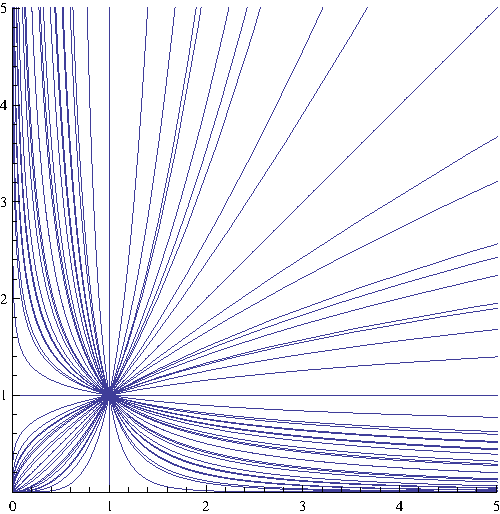
\includegraphics[width=2in]{03-Patterns/support/logspace-picture}

	\item The 3rd and 4th axioms for scalar multiplication fail. 
%	(M1) $k[(a,b)+(c,d)] = k(a+c,b+d) = (2k(a+c),2k(b+d)) = (2ka+2kc,2kb+2kd) = (2ka,2kb)+(2kc,2kd)=k(a,b)+k(c,d)$.
%	(M2) $(j+k)(a,b) = (2(j+k)a,2(j+k)b) = (2ja + 2ka,2jb+2kb) = (2ja,2jb)+(2ka,2kb) = j(a,b)+k(a,b)$.
	(M3) $j(k(a,b)) = j(2ka,2kb)=(2j2ka,2j2kb)=jk(2a,2b)$ instead of $jk(a,b)$.
	(M4) $1(a,b) = (2a,2b)\neq (a,b)$.
	
	
	\item
\begin{enumerate}
	\item 
	Distribution across scalar multiplication fails:  
	$(j+k)(a,b) = (a,(j+k)b) = (a,jb+kb)$ whereas $j(a,b)+k(a,b) = (a,jb)+(a,kb) = (2a,(j+k)b)$ 
	(notice that $a$ is doubled if we multiply first before adding).
	\item  
	Vector addition is not commutative. $(a,b)+(c,d) = (a+c,b)$ while $(c,d)+(a,b) = (a+c,d)$ 
	(the second components are not the same, $b\neq d$.
\end{enumerate}


	\item 
\begin{enumerate}
	\item  Distribution across scalar multiplication fails.
	(M2) $(j+k)(a,b) = ((j+k)^2a,(j+k)b)$ whereas $j(a,b)+k(a,b) = (j^2a,jb)+(k^2a,b) = ((j^2+k^2)a,(j+k)b)$, and $j^2+k^2\neq (j+k)^2$.
	\item  
	Vector addition is not commutative. $(a,b)+(c,d) = (a,d)$ while $(c,d)+(a,b) = (c,b)$.
	
\end{enumerate}


\end{enumerate}



\item \textbf{Vector Subspaces:} 
See chapter 4 problems 13-15, 45-46. Complete at least 13, 15, 46.

\begin{enumerate}
	\item 
		\begin{enumerate}
			\item Yes.  It contains zero, the sum of any two vectors on the $y$ axis is on the $y$ axis, and any scalar multiple of a vector on the $y$ axis is still on the $y$ axis.  The span of $(0,1)$ is the $y$ axis.
			\item No. The zero vector is not on the positive $x$ axis.
			\item No. You cannot times vectors by negative scalars, so it's not closed under scalar multiplication.
			\item Yes. It is the span of $(1,3)$. Lines through the origin are vector subspaces.
			\item No. The line does not contain the zero vector.  It doesn't pass through the origin.
			\item No. It does contain the origin, and is closed under scalar multiplication, but not under vector addition.  The sum $(1,0)+(0,1)=(1,1)$ is not on either axis.
			\item No. Not closed under scalar multiplication. The product $4(1/2,0) = (2,0)$ is not in the set.
		\end{enumerate}


	\item Use theorem \ref{thm subspace iff closed}.
	(1) The zero function is continuous, so zero is in the set. 
	(2) The sum of two continuous functions is a continuous function, so the set is closed under addition.
	(3) A constant times a continuous function is still continuous, so the set is closed under scalar multiplication.
	
	\item Use theorem \ref{thm subspace iff closed}.
	(1) The zero function is a polynomial, so zero is in the set. 
	(2) The sum of two polynomials is a polynomial, so the set is closed under addition.
	(3) A constant times a polynomial is a polynomial, so the set is closed under scalar multiplication.
	
	
	\item 
\begin{enumerate}
	\item 
	(1) The zero function is said to be in the set, so zero is in the set. 
	(2) The sum of two polynomials of degree three must be a polynomial of degree 3 or less, so the set is closed under addition.
	(3) Multiplying a polynomial by a nonzero constant does not change the degree, so the set is closed under scalar multiplication.

	\item The span of the polynomials $\{1,x,x^2,x^3\}$ is $P_3(x)$.  
\end{enumerate}

	\item Let $V$ be the set of 3 by 3 upper triangular matrices.  Show that $V$ is a subspace of the vector space $M_{33}$ of 3 by 3 matrices in 2 ways:
\begin{enumerate}
	\item 
	(1) The zero matrix is upper triangular. 
	(2) The sum of two upper triangular matrices is upper triangular, so the set is closed under addition.
	(3) Multiplying an upper triangular matrix by a constant gives an upper triangular matrix, so the set is closed under scalar multiplication.

	\item 
	The span of 
	$\begin{bmatrix}
	1&0&0\\
	0&0&0\\
	0&0&0
	\end{bmatrix}$,
	$\begin{bmatrix}
	0&1&0\\
	0&0&0\\
	0&0&0
	\end{bmatrix}$,
	$\begin{bmatrix}
	0&0&1\\
	0&0&0\\
	0&0&0
	\end{bmatrix}$,
	$\begin{bmatrix}
	0&0&0\\
	0&1&0\\
	0&0&0
	\end{bmatrix}$,
	$\begin{bmatrix}
	0&0&0\\
	0&0&1\\
	0&0&0
	\end{bmatrix}$,
	$\begin{bmatrix}
	0&0&0\\
	0&0&0\\
	0&0&1
	\end{bmatrix}$
	is the set of upper triangular matrices
  $\begin{bmatrix}
	a&b&c\\
	0&d&e\\
	0&0&f
	\end{bmatrix}$.

	
\end{enumerate}
	\item 
		\begin{enumerate}
			\item 
			Yes. Zero is a symmetric matrix. The sum of two symmetric matrices is symmetric. A constant times a symmetric matrix is symmetric.  Alternatively, the symmetric matrices 
	$\begin{bmatrix}
	a&b\\
	b&c
	\end{bmatrix}$
are spanned by 
	$\begin{bmatrix}
	1&0\\
	0&0
	\end{bmatrix}$
,
	$\begin{bmatrix}
	0&0\\
	0&1
	\end{bmatrix}$
, 
	$\begin{bmatrix}
	0&1\\
	1&0
	\end{bmatrix}$, and hence are a subspace of $M_22$.
			\item	No. The zero matrix is not invertible. 
			\item Yes. Similar to the previous problem related to 3 by 3 matrices.
		\end{enumerate}

	\item 
		\begin{enumerate}
			\item No. The zero polynomial does not have degree 2.
			\item No. The sum of two degree 2 polynomials may be lower in degree.  For example $(x^2) + (x-x^2) = x$. So this set is not closed under addition.
			\item Yes. It is spanned by $\{1,x,x^2\}$
			\item No. Similar to part (b).
		\end{enumerate}

\end{enumerate}




\item \textbf{Spans:} \label{span solutions} \hypertarget{span solutions target}{\hyperlink{span problems target}{(problems link)}}

\begin{enumerate}
	\item 
All but the third have the same row space. The rref of these matrices has the same nonzero rows.


	\item 
All but the third have the same column space. The rref of the transpose of each matrix has the same nonzero rows.

	\item 
		\begin{enumerate}
			\item Yes. The rref is the identity.
			\item No. Only 2 independent columns. Column 3 has coordinates $(3,-1)$.
			\item No. You need at least 3 vectors to span $P_2(x)$.
			\item Yes. There are 3 independent vectors.  The 4th column has coordinates $(1,-1,2)$.
			\item No. Only 2 independent vectors. The coordinates of column 3 are $(1,-1)$, column 4 $(1,2)$.
		\end{enumerate}

	\item 
		\begin{enumerate}
			\item No. You need at least 4 vectors.
			\item Yes.
			\item No. The third polynomial is the sum of the first 2.  There are only 3 independent vectors. 
		\end{enumerate}

	\item 
		\begin{enumerate}
\item 
Yes.

\item 
No.

\item 
No.

\item 
Yes.

		\end{enumerate}
		
\item \textbf{Basis and Dimension:} 
		
\end{enumerate}












\end{enumerate}
\end{multicols}




%%% Local Variables: 
%%% mode: latex
%%% TeX-master: "../linear-algebra"
%%% End: 
